\section{DualReadout}
Most recent update: 2018-07-11 \\
Contact person: John Hauptman (email:  hauptman@iastate.edu)

\subsection{Introduction}
The scientific goal of the RD52/DREAM collaboration~\cite{dreamCollaboration} is to understand the fundamental limitations
to hadronic energy resolution and, in general, the limitations to achieving high-quality calorimetric
performance with Gaussian energy resolution, mean response linearity, and precision robust calibration.

\begin{figure}
  \centering
  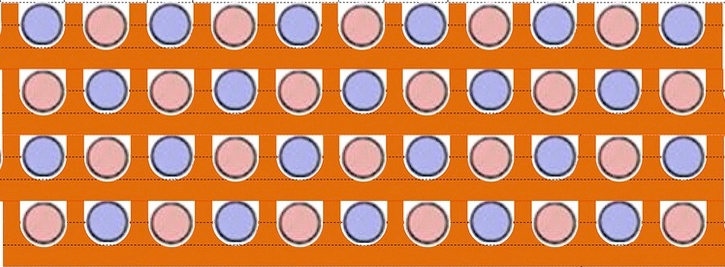
\includegraphics[width=.5\linewidth]{Calorimeter/DualReadout/f32-fibers.jpg} \\
  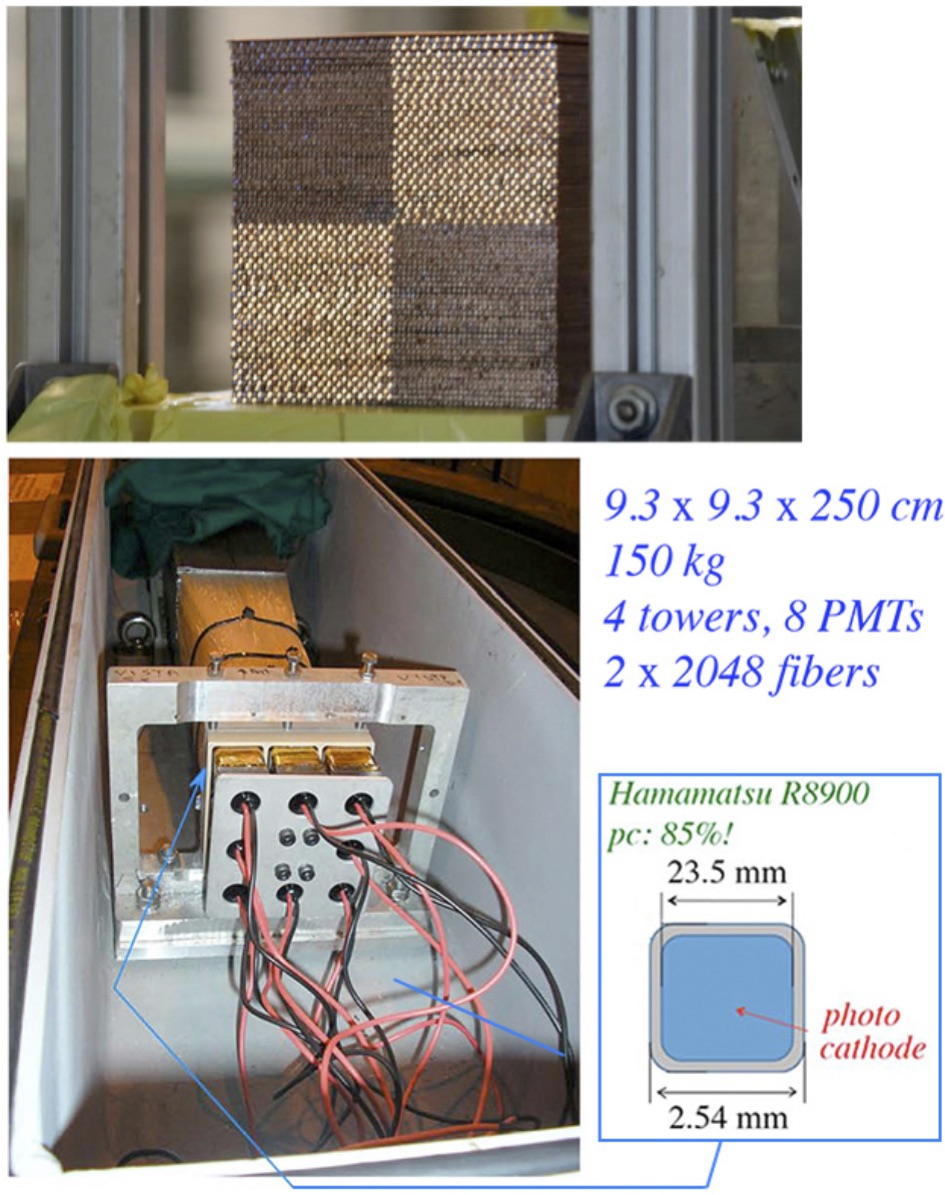
\includegraphics[width=.5\linewidth]{Calorimeter/DualReadout/f33-pisa-module.jpg}
  \caption{Fiber geometry (top) and INFN Pisa copper modules (bottom).}
  \label{fig:pisa}
\end{figure}

Our latest (and final) results indicate that a copper absorber matrix loaded uniformly in volume with 1 mm diameter
fibers of two kinds (scintillating and clear \v{C}er\-enk\-ov fibers) is an excellent choice for a collider detector that 
can reconstruct the four-vectors of $W \rightarrow q\bar{q}$ and  $Z \rightarrow q\bar{q}$ decays.  The simplicity of the construction of such a calorimeter is shown in Fig.~\ref{fig:pisa}.  The fiber-copper geometry is shown at the top.  The upstream beam entry is shown in the middle, and the downstream readout of the separate bundles of  scintillating and \v{C}er\-enk\-ov fibers is shown at the bottom.  This module was built at INFN Pisa.

The essential features of  fiber dual-readout calorimeters are (a) near-perfect optical conduits (fib\-ers)
for extraction of the optical signal from the interior of the calorimeter mass to exterior photo-convert\-ers, 
(b) fine spatial sampling on the mm-scale, (c) dual measurement of scintillation light in scintillating
fibers (all charged particles) and simultaneous \v{C}er\-enk\-ov light in clear fibers (predominantly electromagnetic
particles), (d) nearly absolute fiber-absorber volume uniformity, (e) good lepton identifications, (f) measurement of the neutron content of showers, and (g) equal response to pions and protons (and presumably kaons).

\begin{figure}
  \centering
  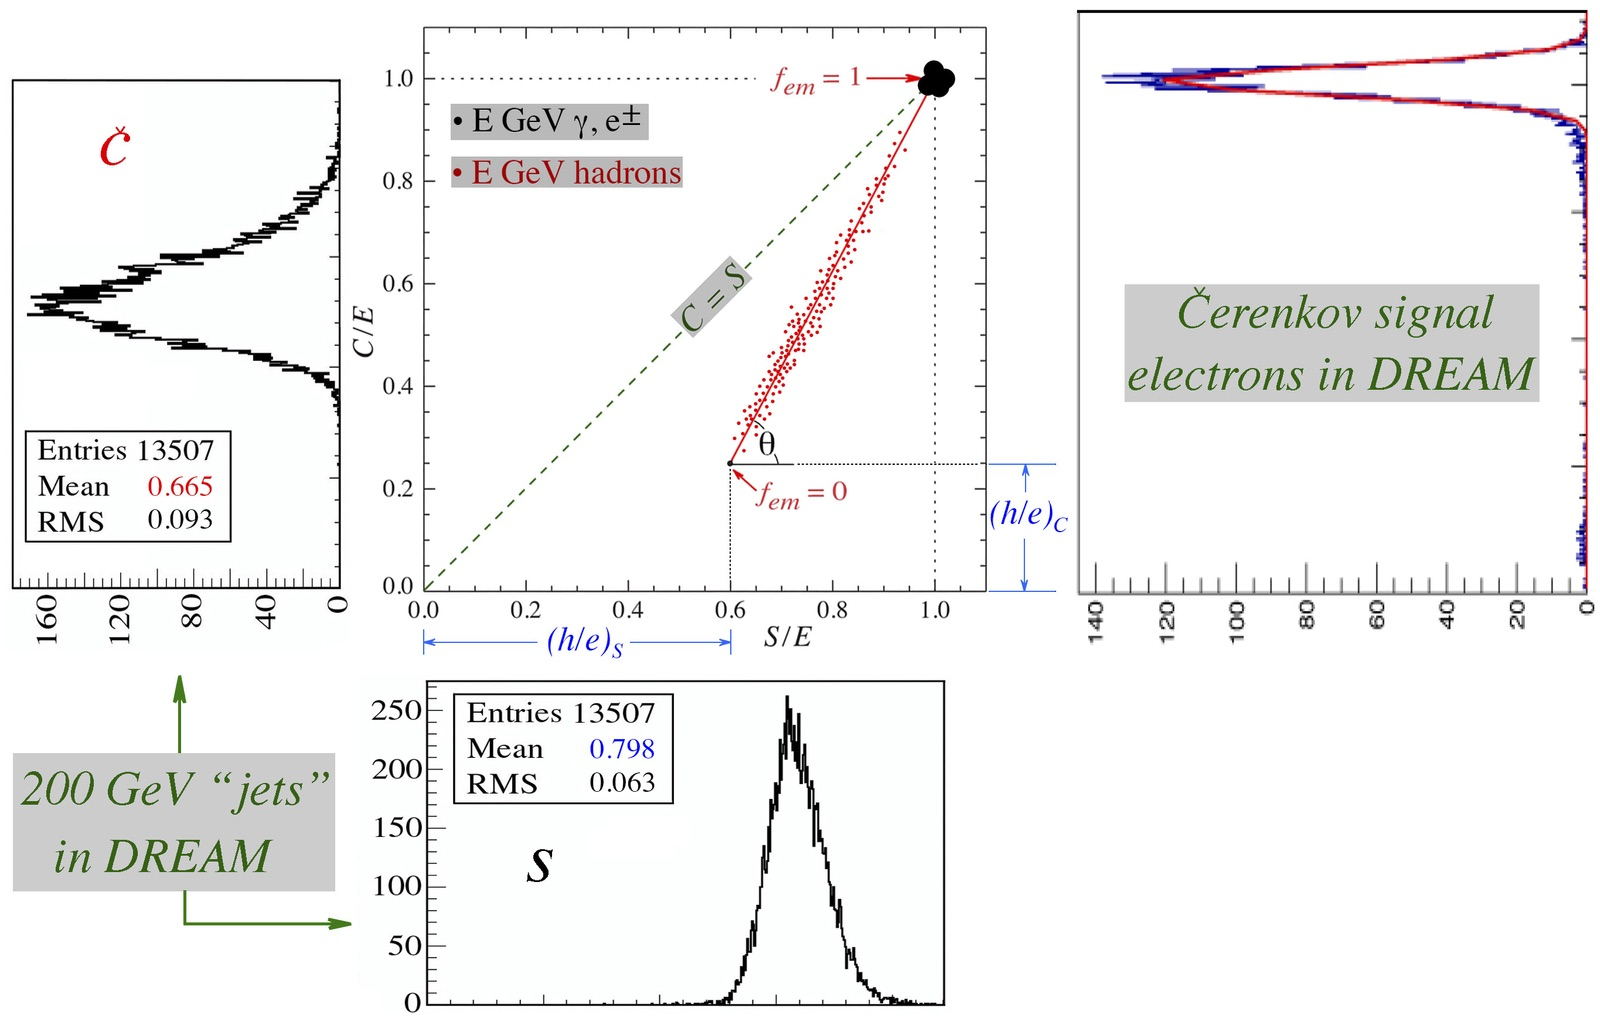
\includegraphics[width=.7\linewidth]{Calorimeter/DualReadout/groom-plot-projs.jpg}
   \caption{Illustration of a dual-readout calorimeter.  Electromagnetic events cluster around $S/E\approx C/E \approx 1$,
   while hadronic events are distributed along the line from $f_{em}$=0 to $f_{em}$ = 1.  The projections onto the $S/E$ and $C/E$
   axes show the resolutions of the corresponding single-readout scintillation sampling and \v{C}er\-enk\-ov sampling calorimeters.}  
   \label{fig:groom}
 \end{figure}
 
 A copper absorber of $10 \lambda_{\text{Int}}$ depth with embedded scintillation ($S$) and \v{C}er\-enk\-ov ($C$) fibers achieves
 all of these goals:  Gaussian hadronic energy response,  linear mean response from 20-300 GeV, 
  robust calibration with single electrons into each geometrical volume, 
  equal response to pions and protons, 
  excellent mass resolution on hadronic decays of the $W$ and $Z$,
  in addition to very good $e^{\pm}$ -  $\pi^{\pm}$  and  $\mu^{\pm}$ -  $\pi^{\pm}$ separation.  
  
About 30 dual-readout papers are published in {\it Nucl. Intrs. Meths.}, {\it Rev. Sci. Instr.}, and {\it JINST}, including
dual-readout in several crystals, in a planar geometry, as well as in several fiber geometries. We have built
and tested both Pb-based and Cu-based dual-readout fiber modules.   

Hadronic events of energy $E$ (initiated by $\pi^{\pm}, K, p$, or jets) shower in this copper-fiber structure and develop scintillation ($S$) and 
\v{C}er\-enk\-ov ($C$) signals given by the sum of their respective electromagnetic ($f_{em}$) and non-electromagnetic ($1-f_{em}$) components:

\begin{displaymath}
  S = E [ f_{em} + (1 - f_{em}) \cdot \eta_S ]
\end{displaymath}

\begin{displaymath}
  C = E [ f_{em} + (1 - f_{em}) \cdot \eta_C ]
\end{displaymath}

\noindent where the $\eta_S$ and $\eta_C$ are constants determined by the structure of the calorimeter (number of S fibers, number of \v{C}er\-enk\-ov fibers, volume ratios of fiber to copper, etc.), and are the ratios of the mean hadronic response to the mean electromagnetic response.  The fraction of each event that is electromagnetic, $f_{em}$, is measured directly event-by-event by the ratio $C/S$, and this electromagnetic fraction $f_{em}$ ~ varies from $f_{em}$ = 0 at $S/C = (1-\eta_S)/(1-\eta_C)$ to $f_{em}=1$ at $S/C=1$.

All hadronic events fall on the line joining $f_{em}=0$ to $f_{em}=1$, as illustrated in Fig. \ref{fig:groom}.  The projections 
onto the $S/E$ and $C/E$   axes show the resolutions of the corresponding single-readout scintillation sampling and \v{C}er\-enk\-ov sampling calorimeters, while the dual-readout resolution is the projection along the perpendicular to this line, and
  this shows the fundamental reason that dual-readout calorimeters have intrinsic good energy resolution.

\subsection{Recent Milestones}

\subsubsection{Neutrons in GEANT} 
\label{sec:geant}  

\begin{figure}
 \centering
 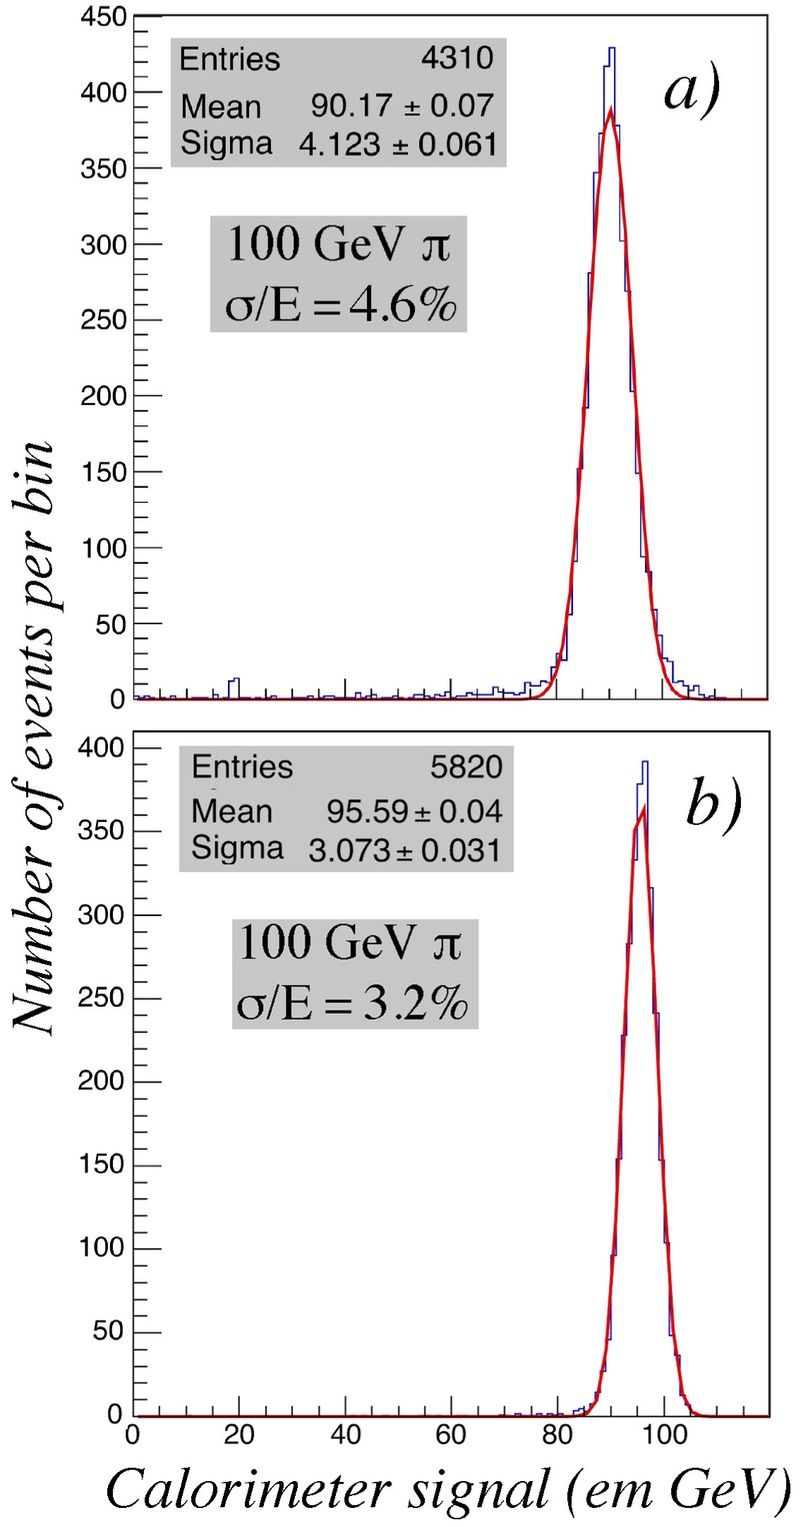
\includegraphics[width=.5\linewidth]{Calorimeter/DualReadout/f41-geant.jpg}
 \caption{(a) GEANT4 regular hadronic simulation compared to the (b) GEANT ``high precision'' simulation.}
 \label{fig:hp}
\end{figure}
In the early days of DREAM ({\it circa} 2004), the GEANT3 simulations did not accord well with the DREAM data.  Recently, Sehwook Lee
at Kyungpook National University has simulated the RD52 calorimeters (both the small modules we've built and a large
5-6 tonne module we have not been able to build) with both the regular GEANT4 and the ``high precision'' version of GEANT4.  The difference in simulated dual-readout calorimeter response is shown in Fig.~\ref{fig:hp}.  This is a huge difference in energy resolution, from 4.6\% (regular GEANT4) down to 3.2\% (high precision GEANT4), due solely to the version of GEANT4 being used. It is clear that neutron measurement is critical to 
dual-readout for the same reason it is critical to a compensating calorimeter.

This is a large difference, and we believe it derives from a more correct treatment of the neutrons and their transport, including the proper treatment of neutron and proton spallation processes and the the treatment of binding energy losses during the violent disassembly of a nucleus.   Note that in  Fig.~\ref{fig:hp}(a) the mean is 90.17 GeV (resolution 4.6\%) out of 100 GeV incident pion, and in Fig.~\ref{fig:hp}(b) the mean energy is 95.59 GeV (resolution 3.2\%). I suspect that a further improved treatment of neutrons will recover this additional 4\% in energy with a consequent improvement of the energy resolution. On 4th, we used FLUKA which is known to treat neutrons explicitly correctly (LANL codes) and we achieved the correct mean response and a resolution at 100 GeV of about 2.9\%.

Note that this single result (in the absence of a constant term) implies a hadronic energy resolution of
\begin{displaymath}
  \sigma / E \approx 32\% / \sqrt{E}
\end{displaymath}
Nota bene: it is easy to get a small constant term in a simulation, but much more difficult in an actual device.

\subsubsection{Equal response to pions and protons}
\label{sec:pi-p}

\begin{figure}
 \centering
 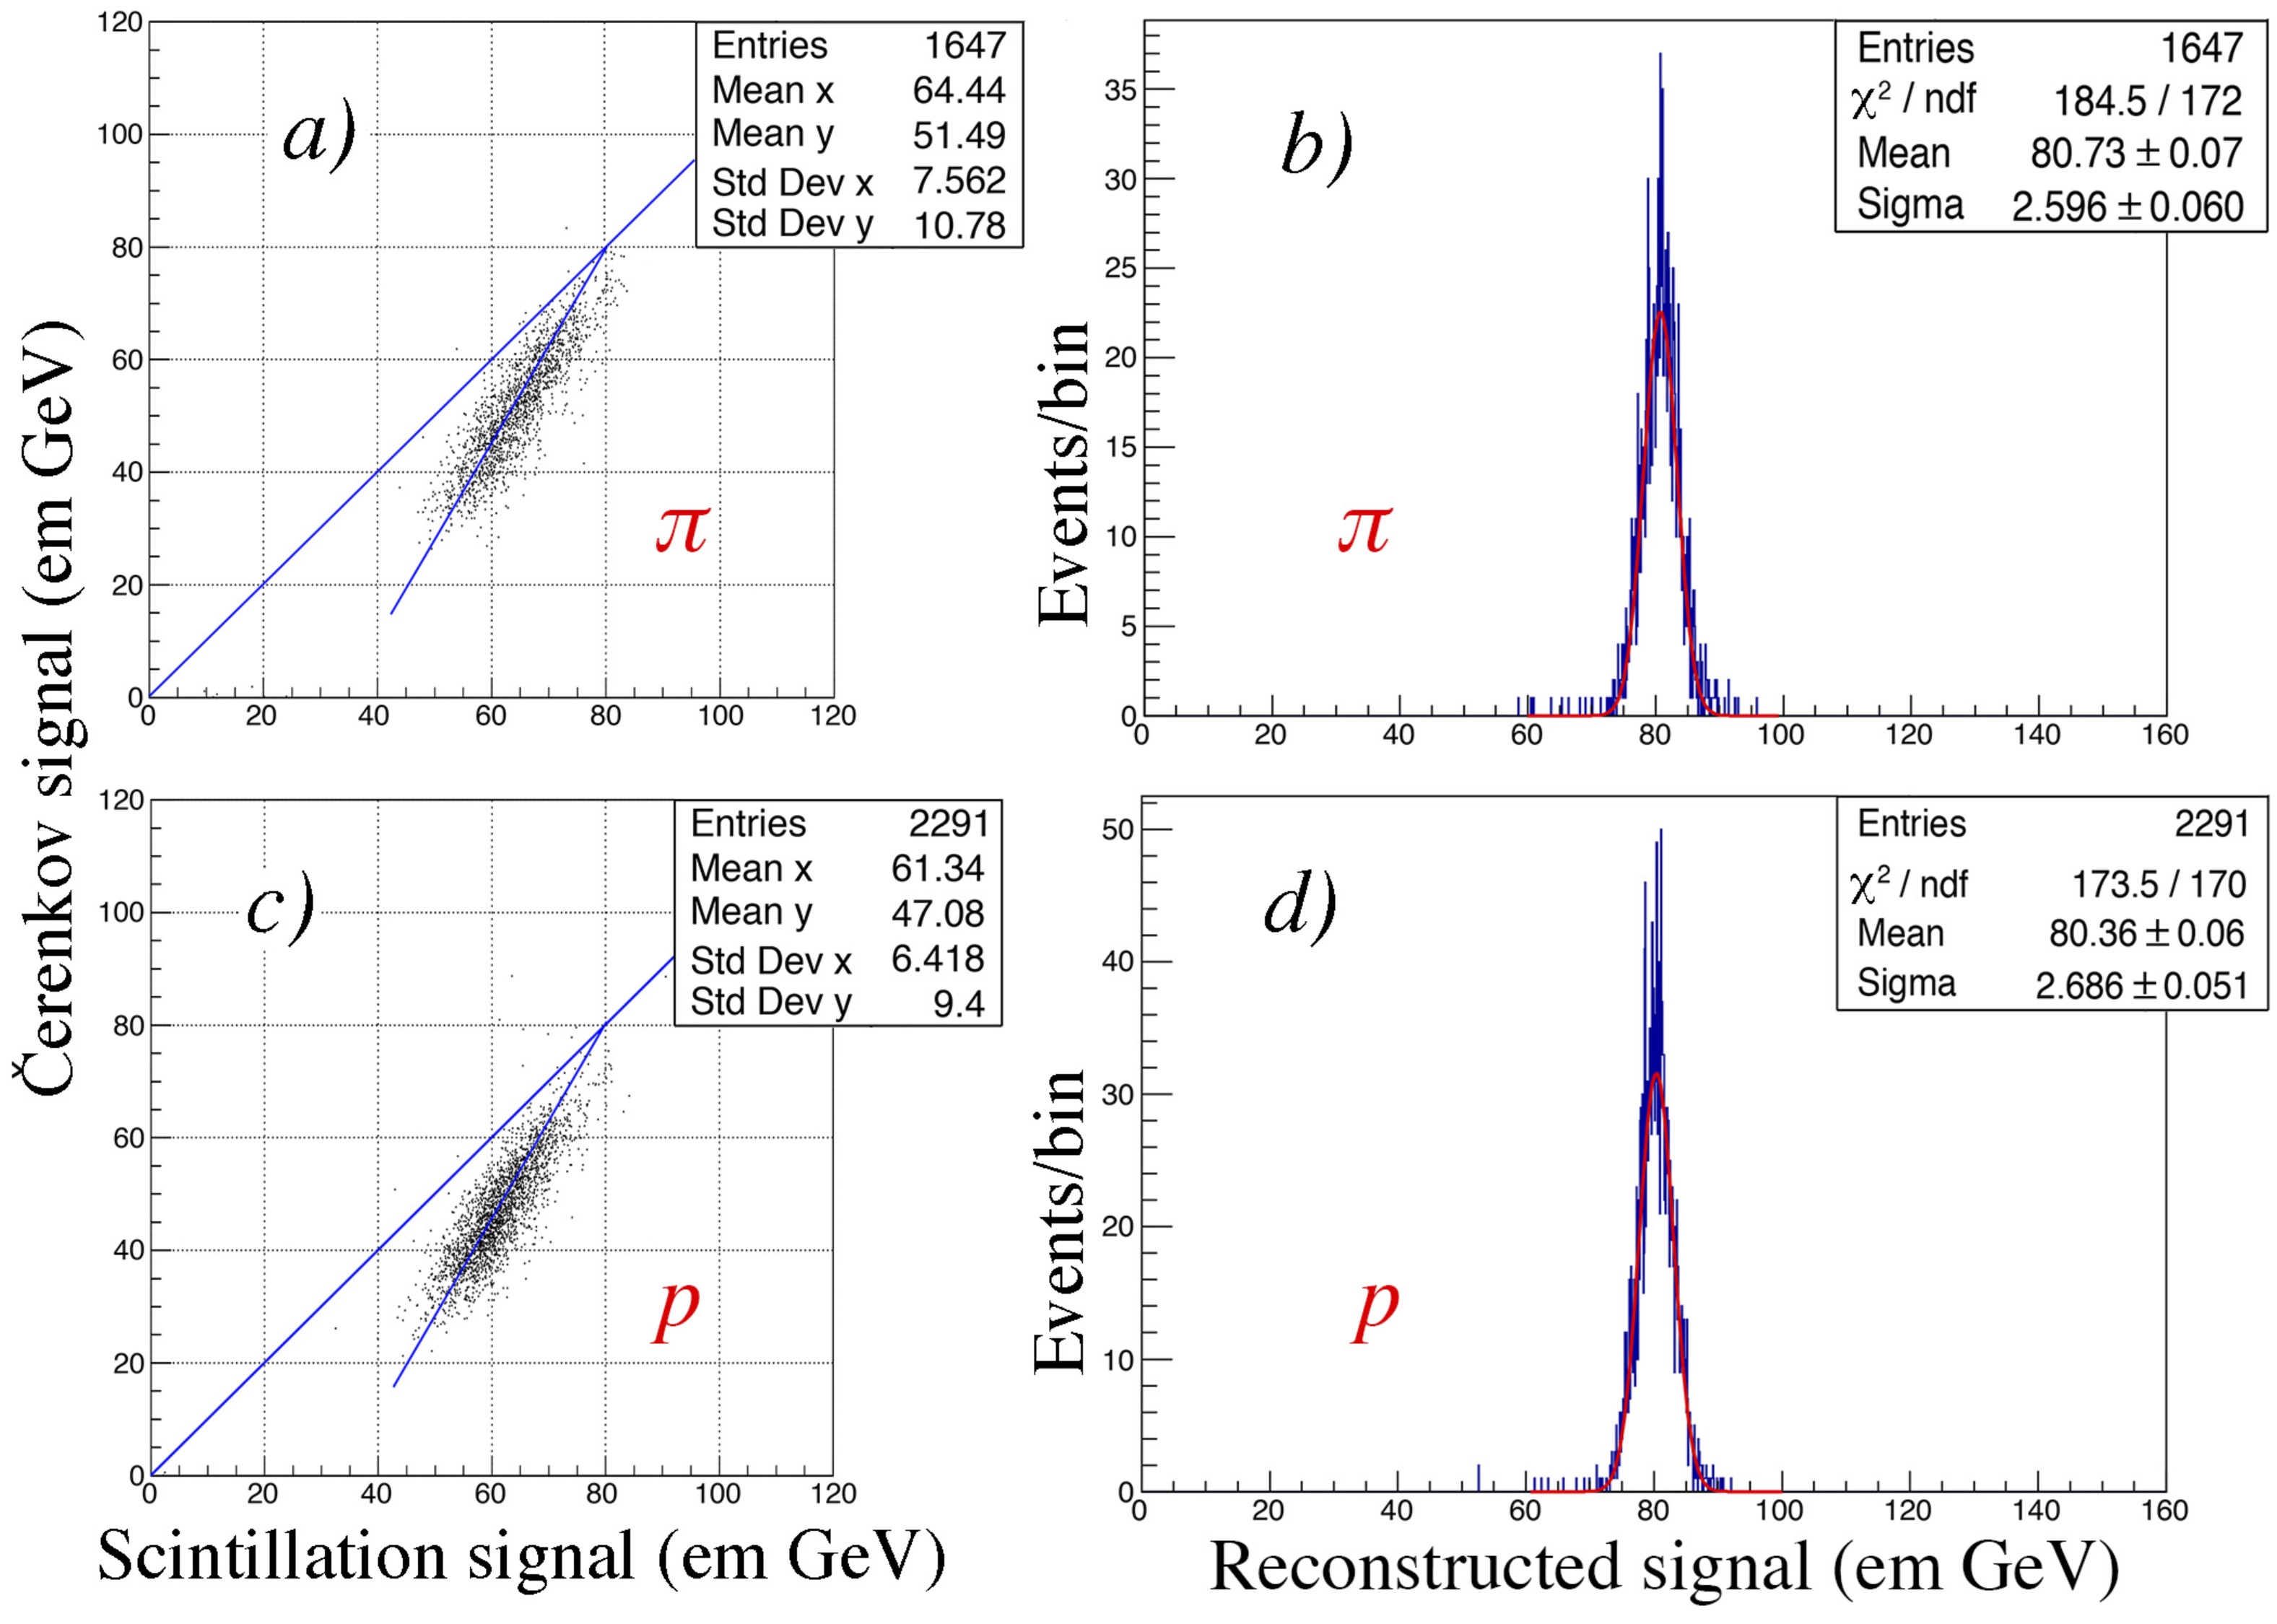
\includegraphics[width=.5\linewidth]{Calorimeter/DualReadout/f42-pion-proton.jpg}
 \caption{Dual-readout of pion and proton responses.}
 \label{fig:pi-p}
\end{figure}

In a dual-readout calorimeter, hadronic events with differing
electromagnetic fraction are distributed along the line in Fig.~\ref{fig:groom} between $f_{em}=0$ and $f_{em}=1$.  Proton-initiated
showers have fewer pions, and fewer neutral pions, due to baryon conservation, and therefore a lower response in both $S$ and $C$ but,
nevertheless, the dual-readout solution is the same for both as seen in Fig.~\ref{fig:pi-p}.  This is important for jet energy resolution as the baryon  
content of jets varies.  The same will likely be true of kaon-initiated showers, but we have not measured this. 

\subsubsection{Simulated energy resolution}
\label{sec:Eres}  

The same simulation of high-precision GEANT4 was run at pion energies of 50, 80, 90, 100 and 200 GeV in a large
copper-fiber calorimeter with Gaussian fitted  means and resolutions, displayed in Fig.~\ref{fig:eres} and in Table~\ref{tab:dream:pionEnergies}.
\begin{table}
  \centering
\begin{tabular}{ r r r }
$E_{\rm beam}$   &  Mean         &  $\sigma/E$ \\
   (GeV)    &   (GeV)       &   \\
\hline
 & & \\
 50    &    47.85   & 4.4 \% \\
 &&\\
 80   & 76.46     &  3.5 \% \\
 &&\\
 90  & 85.95    &   3.4 \% \\
 &&\\
 100  & 95.42  &  3.2 \% \\
 &&\\
 200  & 190.2  &  2.5 \% \\
 &&\\
 \end{tabular}
 \caption{HIgh precision GEANT4 simulation of a copper-fiber dual-readout calorimeter for incident $\pi^-$ energies of 50, 80, 90, 100 and 200 GeV.  The energy resolution can be characterized by $\sigma/E \approx 31-35 \% / \sqrt{E}$.}
 \label{tab:dream:pionEnergies}
\end{table}

 It is observed that the response is Gaussian and linear, although the mean response is low by about 5\%.  This (I believe) is due to an insufficiently accurate treatment of the neutrons in GEANT4 (high precision version, FTFP\_BERT\_HP).
 
 It is clear that these dual-readout calorimeters can achieve (in simulation) a raw energy resolution of about $\sigma/E \approx 30\% / \sqrt{E}$ with a negligible constant term.  

\begin{figure}
 \centering
 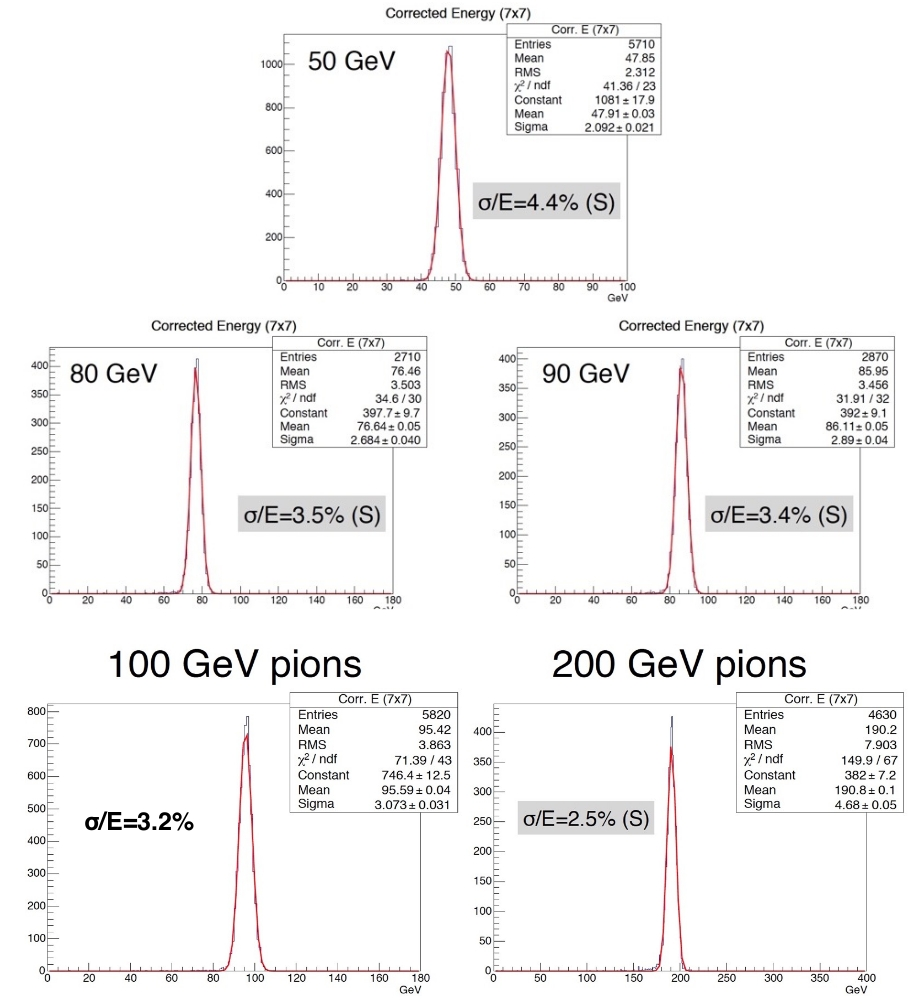
\includegraphics[width=0.5\linewidth]{Calorimeter/DualReadout/eres.jpg}
  \caption{Energy resolution from GEANT-HP at 50, 80, 90, 100, and 200 GeV.}
  \label{fig:eres}
\end{figure}


\subsubsection{$W$ and $Z$ hadronic decays}

The main goal of a electron-positron collider at  Higgs and top production running is the direct and high-precision reconstruction of  $W \rightarrow q\bar{q}$ and  $Z \rightarrow q\bar{q}$ decay four-vectors.   This is obvious, and will increase the efficiency of $W,Z$ events for physics analysis by large factors of 10-100, depending on the final states.

We have used DREAM data events taken in the ``interaction jet'' trigger to assembly di-jet events distributed as $W$ and $Z$ Breit-Wigner line shapes by adjusting the space angle between the two measured beam particles, $\theta_{12}$, 
\begin{displaymath}
   M^2 = 2 E_1 E_2 ( 1 - \cos \theta_{12}),
\end{displaymath}
then using the measured hadronic showers in the two data events to reconstruct the energies, $E_1$ and $E_2$, and the space angle between the two showers.  The results of this exercise on event files at beam energies of 50, 100, and 200 GeV are shown in Fig.~\ref{fig:wz}, where the $W$ events and the $Z$ events are superposed, and these three beam energy files allow the reconstruction of simulated $W/Z$ laboratory energies of 100, 150, 200, 250, 300, and 400 GeV.  

\begin{figure}
 \centering
 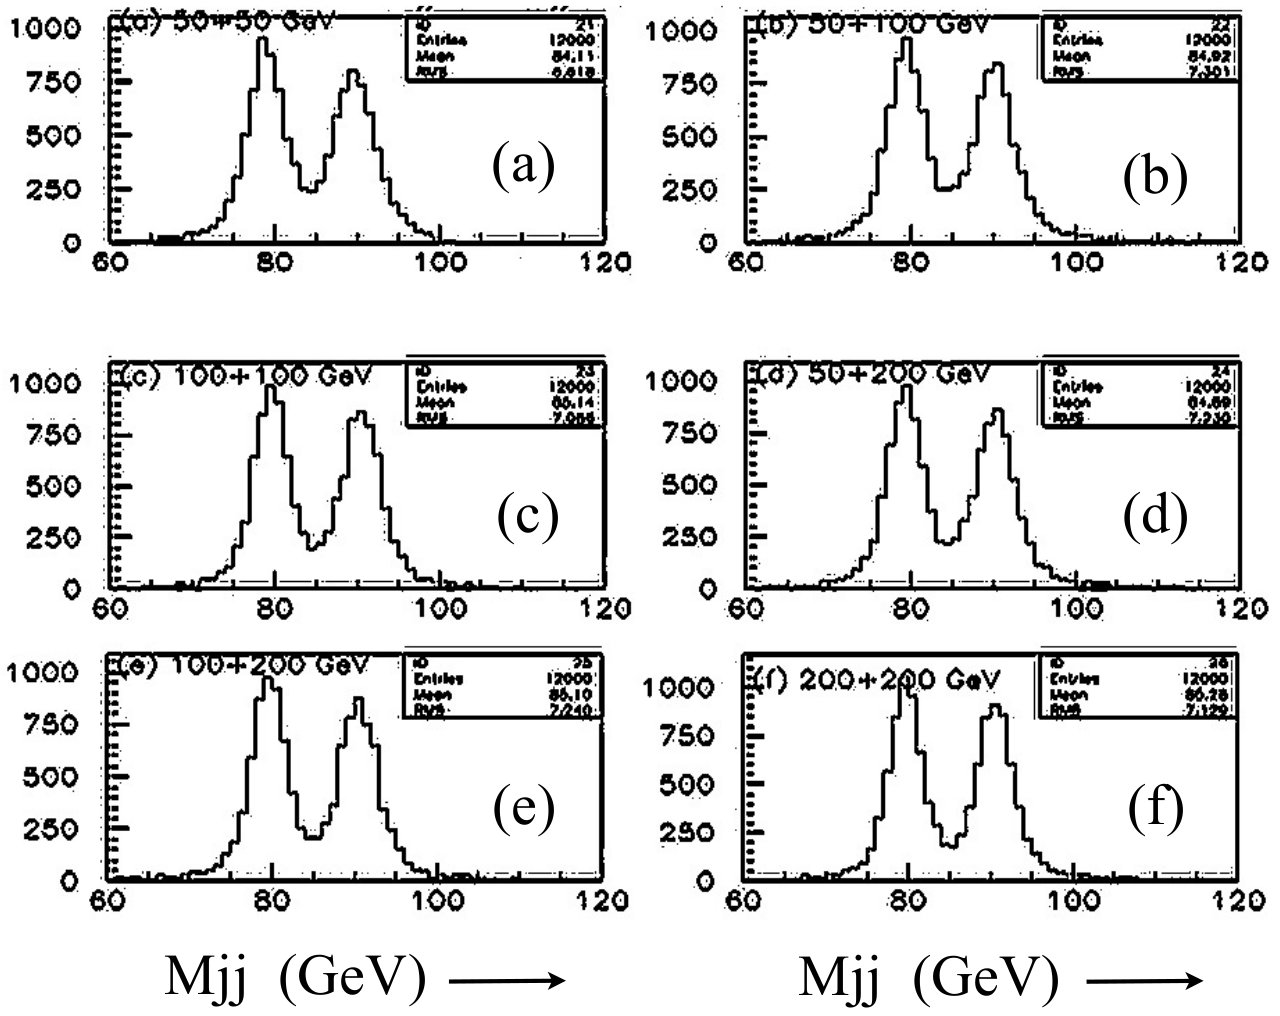
\includegraphics[scale=0.45]{Calorimeter/DualReadout/WZ-Dream-data-all.jpg}
  \caption{Hadronic decays $W \rightarrow q\bar{q}$ and  $Z \rightarrow q\bar{q}$ assembled for DREAM beam events as described in the text.}
  \label{fig:wz}
\end{figure}

\subsection{Engineering Challenges}

There are two main challenges before a dual-readout calorimeter can be incorporated into a collider detector~\cite{Hauptman_CEPC}:

\begin{description}

\item Construct wedges (trapezoids) so that a $4 \pi$ geometrical volume can be filled hermetically. This has been done in the 4th concept design~\cite{fourthConcept} as shown in Fig.~\ref{fig:hcalor}, and is being done again in the CEPC design (R. Ferrari).  This problem was also addressed with respect to the SPACAL calorimeter in RD1 at CERN.

\item Develop photo-converters that will work in a magnetic field.  We have tested SiPMs (see M. Caccia, CEPC meeting, May 2018).  In addition to eliminating the fiber bundles at the rear of the calorimeter (Fig.~\ref{fig:pisa}), SiPMs would allow on to build an ``em'' section in front of a ``hadronic'' section.  We do not believe this is necessary for either lepton ID or general calorimeter performance, but it becomes an option. 
 
\end{description}
 
\begin{figure}
  \centering
  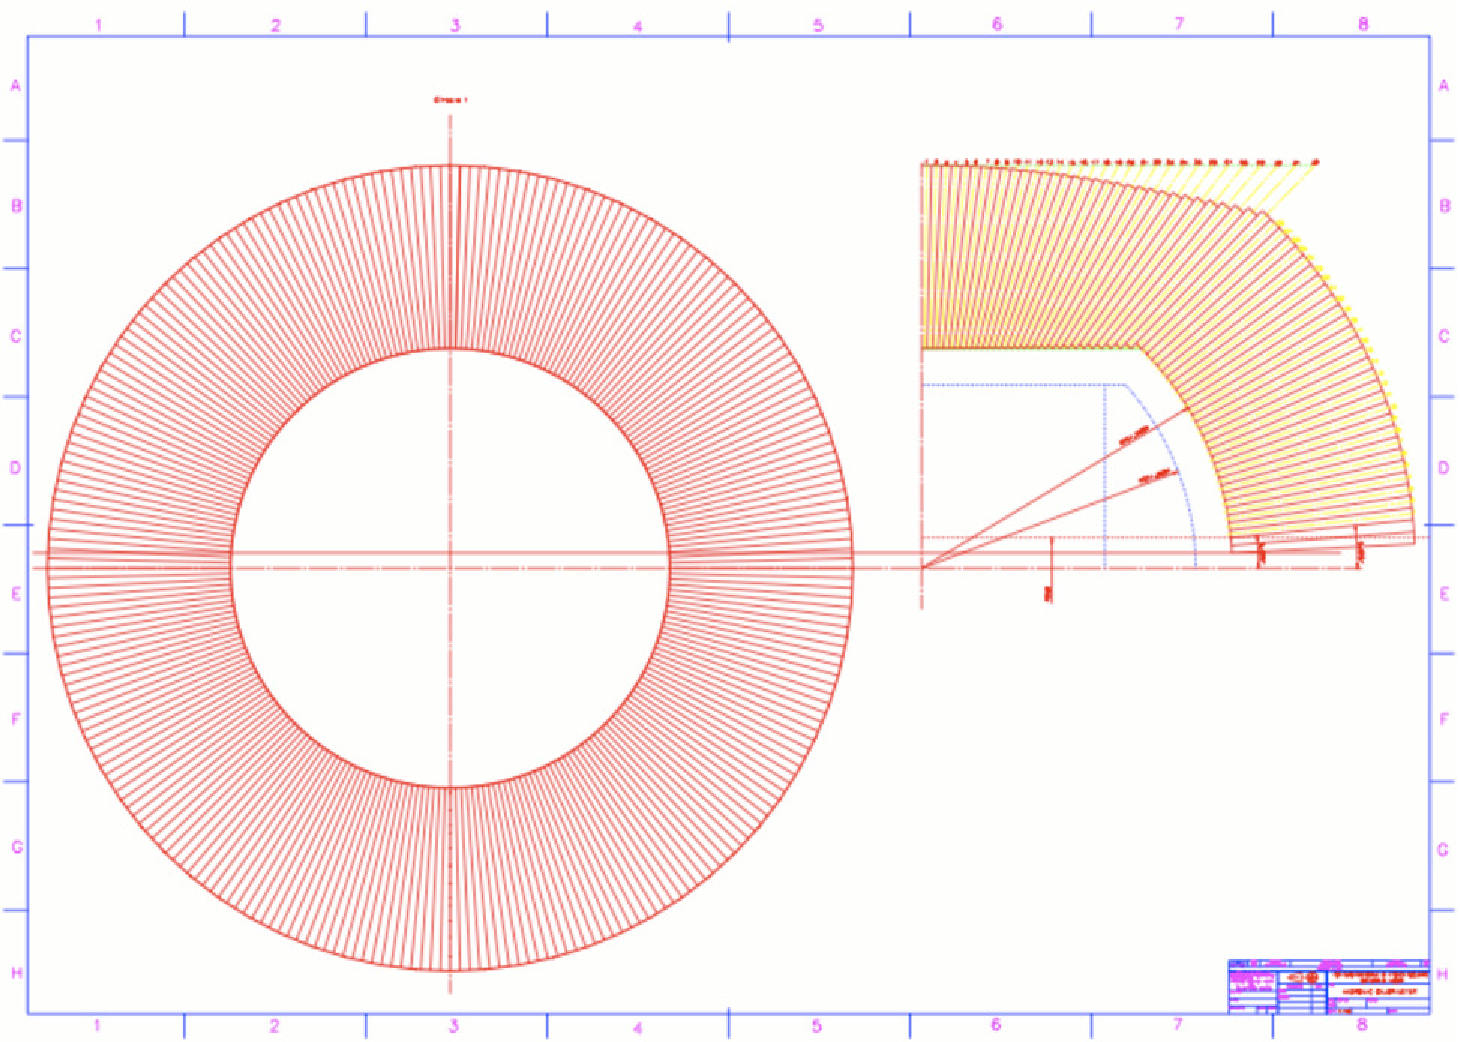
\includegraphics[width=0.5\linewidth]{Calorimeter/DualReadout/hcalor}
  \caption{The 4th Concept~\cite{fourthConcept} calorimeter geometry. This geometry was fully simulated. }
  \label{fig:hcalor}
\end{figure}

\subsection{Future Plans}

We have no future plans, since RD52 has been completed. See all RD52 papers~\cite{dreamCollaboration}. The only possible plan would be to build a 5-6 tonne copper-fiber module to test for all aspects at a collider, e.g., wedges, $4 \pi$ geometry, energy resolution, particle ID, and photo-converter readout. 
